\begin{mainquestion}{nmosbias}{NMOS Bias Point Calculation}

Consider the circuit below, where $k_{n} = 5\ \frac{\text{mA}}{V^{2}}$ and $V_{tn} = 0.8\ \text{V}$.

\begin{center}
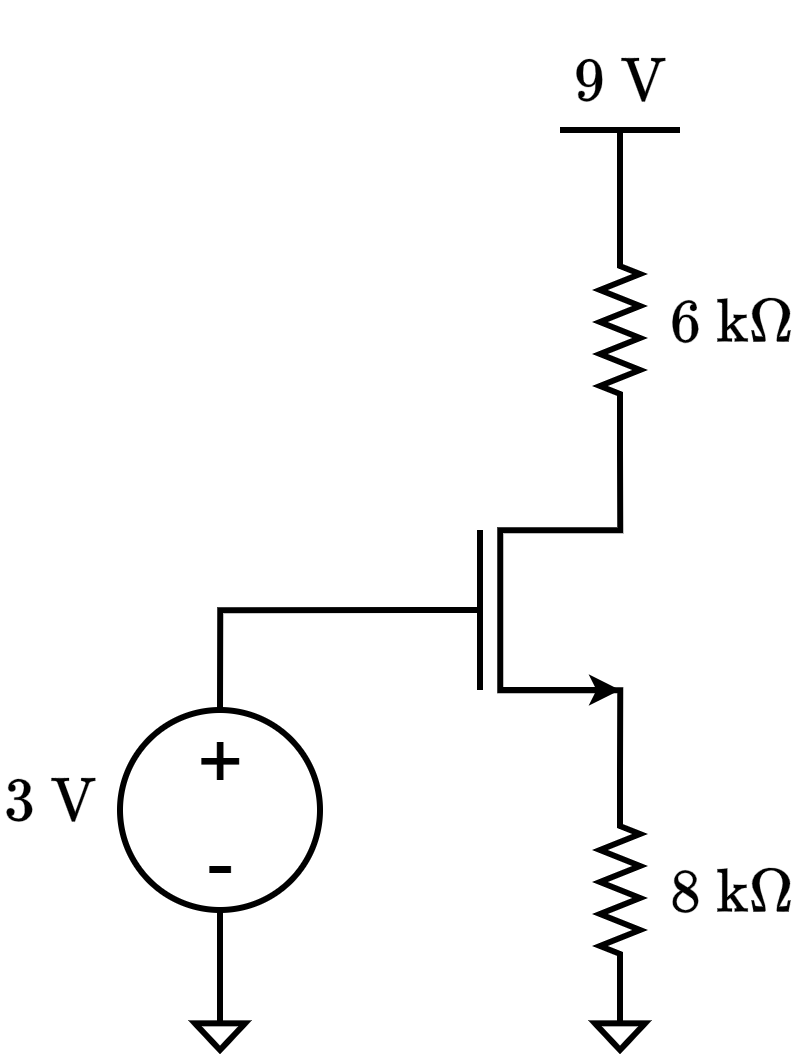
\includegraphics[height=4in]{questionbank/transistors/nmos_bias/v0/circuit.png}
\end{center}

\begin{partquestion}{findvs}{Find the drain and source voltages for the circuit.}
\begin{answer}
We make an assumption that we are operating in the saturation region, and if we find a contradiction, we will adjust our assumption. The current $i_{D}$ (we will measure in mA) flows from drain to source in NMOS, so we expect the same current through $R_{D}$ and $R_{S}$. We then have:

\[
i_{D} = \frac{V_{DD} - V_{D}}{6} = \frac{V_{S} - 0}{8}
\]

We also know in saturation, the current is given as:

\begin{align}
    i_d &= \frac{1}{2} k_n (v_{GS} - V_{t})^2 \\
    &= \frac{1}{2} k_n (v_G - V_S - V_{t})^2 \\
    &= \frac{1}{2} (5) (3 - V_S - 0.8)^2 \\
    &= \frac{5}{2}(2.2 - V_S)^2 \\
\end{align}

Since $i_{D} = \frac{1}{8}V_{S}$, we can write:

\begin{align}
    \frac{1}{8}V_S &= \frac{5}{2}(2.2 - V_S)^2 \\
    &= 12.1 - 11V_S + 2.5V_S^2 \\
    0 &= 12.1 -11.125V_S + 2.5V_S^2
\end{align}

which has two possible solutions, $V_{S} = 2.558\ \text{V}$ and $V_{S} = 1.892\ \text{V}$. Since $V_{D} = V_{DD} - \frac{6}{8}V_{S}$, this results in $V_{D} = 7.081\ \text{V}$ and $V_{D} = 7.581\ \text{V}$ respectively. In saturation, we have a condition that $v_{DS} > v_{GS} - V_{t}$ that we will want to validate. The first solution gives $v_{DS} = V_{D} - V_{S} = 7.081 - 2.558 = 4.524\ \text{V}$ and $v_{GS} - V_{t} = V_{G} - V_{S} - V_{t} = 3 - 2.558 - 0.8 = -0.358\ \text{V}$. Because this last value is negative, the transistor would need to be in cutoff which contradicts our original assumption. The second solution gives $v_{DS} = V_{D} - V_{S} = 7.581 - 1.892 = 5.688\ \text{V}$ and $v_{GS} - V_{t} = V_{G} - V_{S} - V_{t} = 3 - 1.892 - 0.8 = 0.308\ \text{V}$, which is a valid solution for saturation since $5.688 > 0.308$. Hence $V_{D} = 7.581\ \text{V}$ and $V_{S} = 1.892\ \text{V}$ are the bias points.
\end{answer}
\end{partquestion}

\begin{partquestion}{findcurrents}{Find the gate current and the drain current for the circuit under the same operating conditions.}
\begin{answer}
We expect no gate current in a MOSFET, so $i_{G} = 0$. For the drain current:

\[
i_{D} = \frac{V_{S}}{8} = \frac{1.892\ \text{V}}{8\ \text{k}\Omega} = 0.237\ \text{mA}.
\]
\end{answer}
\end{partquestion}

\end{mainquestion}
